\documentclass[12pt, a4paper]{ctexart}

\usepackage{amsmath}
\usepackage{array}
\usepackage{appendix}
\usepackage{listings}
\usepackage{xcolor}
\usepackage{fontspec}
\usepackage{underscore}
\usepackage{graphicx}
\usepackage{subfigure}
\usepackage{multirow}
\setmonofont{Consolas}
\lstset{
	breaklines=true,
	language = C++, 
	numbers=left,
	backgroundcolor=\color{red!0!green!25!blue!25},%代码块背景色为浅灰色
	rulesepcolor= \color{gray}, %代码块边框颜色
	numberstyle= \small,%行号字体
	frame=shadowbox%用方框框住代码块
	frame=single
}

\title{间断有限元第四次作业报告}
\author{九所 $\quad$ 韩若愚}
\date{2022.4.26}
\begin{document}
	\maketitle
	
	\tableofcontents
	
	\section{题目}
	Consider the Burgers' equation
	\begin{equation*}
	\begin{cases}
	& u_t + (\frac{u^2}{2})_x = 0, \quad -1 \leq x \leq 1\\
	& u(x,0) =\frac{2}{3} + \frac{1}{3} \sin(\pi x)
	\end{cases}
	\end{equation*}
	with periodic boundary condition. Code up the DG scheme for $P^1$ and $P^2$, together with 2nd and 3rd order SSP R-K method in time, respectively. Use uniform meshes in space. Put in a) TVD limiter, b) TVB limiter and c) MPP limiter, respectively. For each limiter, 
	
	1. Take the finial time at $T = 0.4$. Show error tables of the $L^2$ error and $L^\infty$ error.
	
	2. Take $T = 1.5$. Show pictures of the exact solution and the numerical solution.
	
	\section{算法}
	
	\subsection{真解}
	
	由于方程是Burgers方程,所以真解$u$沿特征线$ \frac{dx}{dt} = u$不变。而特征线的斜率刚好是$u$,所以特征线是直线。于是真解为$u(x,t) = u(x- u(\xi,0)t,0)$,其中$\xi$为经过点$(x,t)$的特征线与$t=0$的交点。这个真解是隐式给出的,为了得到真解,需要得到经过点$(x,t)$的特征线的斜率$u(\xi,0)$。
	
	可以使用牛顿迭代法求$\xi$。因为$(x,t)$和$(\xi,0)$在同一条直线上,特征线方程$x = u(\xi,0)t+\xi$可改写为:
	$$
	f(\xi) := x - u_0(\xi) t - \xi = 0
	$$
	其中$u_0(x) = u(x,0)$。于是可以构造迭代公式:
	$$
	\xi^{(n+1)} = \xi^{(n)} - \frac{f(\xi^{(n)})}{f'(\xi^{(n)})}
	$$
	其中$\xi^{(n)}$表示第$n$个迭代值。
	
	\subsection{DG格式}
	
	首先对单元$[-1,1]$ 进行均匀剖分。假设将区间均匀剖分为$n$份,令:
	\begin{equation}
	0 = x_{\frac{1}{2}} < x_{\frac{3}{2}} < \dots < x_{n-\frac{1}{2}} < x_{n+\frac{1}{2}} = 1
	\end{equation}
	则第$j$个区间为:$ I_j = [x_{j- \frac{1}{2}}, x_{j + \frac{1}{2}}]$,每个区间的长度都为$h = \frac{2}{n}$。记$x_{j+1/2}^- = \lim_{x \in I_j, \, x \to x_{j+1/2}} \, x, \  x_{j+1/2}^+ = \lim_{x \in I_{j+1}, \, x \to x_{j+1/2}} \, x$。
	
	假设对固定的时间$t$,所求数值解$u_h$存在的空间为:$ V_h^k := \{ v : \  v|_{I_j} \in P^k(I_j), j = 1, \dots, N \}$,其中$k$为给定常数,$P^k(I_j)$为定义在$I_j$上的最高次项不超过$k$次的多项式空间。并假设检验函数$v \in V_h^k$,用$v$乘以方程两端并在$I_j$上积分。由于方程中通量函数$f(u) = \frac{u^2}{2}$是非线性的,在构造数值格式时需要要求当$k = 0$时,格式退化为一阶单调FD格式,于是空间离散后的半DG格式为:
	\begin{equation}
	\begin{split}
	& \int_{I_j} u_t v \, dx - \int_{I_j} (\frac{u^2}{2}) v_x \, dx\\
	& + \hat{f}_{j+1/2} v(x_{j+1/2}^-) - \hat{f}_{j-1/2} v(x_{j-1/2}^+) = 0, \quad j = 1,\dots,N
	\end{split}
	\label{1}
	\end{equation}
	其中$\hat{f}_{j+1/2}$是单调数值通量,保证在$k=0$时格式退化为1阶单调格式。$\hat{f}_{j+1/2} = \hat{f}(u_{j+1/2}^-, u_{j+1/2}^+)$。
	
	在$I_j$上取定一组$P^k(I_j)$的基底$\{ \phi_j^l \}_{l=0}^k$,则数值解$u_h$在$I_j$上表示为:$u_h(x,t) = \sum_{j=1}^N \sum_{l=0}^k \, u_j^l(t) \, \phi_j^l(x)$,求解$u_h$即求解系数$u_j^l, \, j=1, \dots, N, \, l=0, \dots, k$。令检验函数$v = \phi_j^m, \, m=0, \dots, k$,则方程组(\ref{1})变为:
	\begin{equation}
	\begin{split}
	& \sum_{l=0}^k \int_{I_j} \phi_j^l \phi_j^m \, dx \, u_j^l - \frac{1}{2}\sum_{p,q=0}^k \int_{I_j} \phi_j^p \phi_j^q (\phi_j^m)_x \, dx \, u_j^p u_j^q \\
	& + \hat{f}(\sum_{l=0}^k u_j^l \phi_j^l(x_{j+1/2}),u_{j+1/2}^+) \phi_j^m(x_{j+1/2})\\
	& - \hat{f}(u_{j-1/2}^-, \sum_{l=0}^k u_j^l \phi_j^l(x_{j-1/2} )) \phi_j^m(x_{j-1/2}) = 0, \quad j = 1, \dots,N
	\end{split}
	\label{2}
	\end{equation}
	这是关于向量$\textbf{u}_j = (u_j^0,\dots, u_j^k)$的$m$维方程组。
	
	为便于求解,假设参考单元$I = [-1,1]$,对每个单元$I_j$都有一个到$I$的微分同胚$\Phi_j : I_j \to I$,$ \xi := \Phi_j(x) = \frac{2}{h} (x - x_{j-1/2}) - 1$。在参考单元上取定一组$P^k(I)$的基底$\{\phi^l\}_{l=0}^k$,则由$\Phi_j$将$\phi^l$拉回到$I_j$上得到的函数组$\{(\Phi_j^{-1})^* \phi^l\}$也是$P^k(I_j)$的基底,不妨就设为$\{\phi_j^l\}$。于是每个单元$I_j$上的计算都可以在$I$上进行,方程组(\ref{2})变为:
	\begin{equation}
	\begin{split}
	&  \frac{h}{2} \sum_{l=0}^k \int_I \phi^l \phi^m \, d\xi \, u_j^l -\frac{1}{2} \sum_{p,q=0}^k \int_I \phi^p \phi^q (\phi^m)_\xi \, d\xi \, u_j^p u_j^q \\
	& + \hat{f}(\sum_{l=0}^k u_j^l \phi^l(1),u_{j+1/2}^+) \phi^m(1)\\
	& - \hat{f}(u_{j-1/2}^-, \sum_{l=0}^k u_j^l \phi^l(-1)) \phi^m(-1) = 0, \quad j = 1, \dots,N
	\end{split}
	\label{3}
	\end{equation}
	其中$u_{j+1/2}^+ = \sum_{l=0}^k u_{j+1}^l \phi^l(-1)$,$u_{j-1/2}^- = \sum_{l=0}^k u_{j-1}^l \phi^l(1)$,$j$为循环指标。
	
	(\ref{3})可以写为向量形式:
	$$
	\frac{h}{2} A \frac{d}{dt} \textbf{u}_j = \frac{1}{2} \textbf{u}_j B \textbf{u}_j - C_j
	$$
	\begin{equation}
	\frac{d}{dt} \textbf{u}_j = \frac{2}{h} A^{-1} (\frac{1}{2} \textbf{u}_j B \textbf{u}_j - C_j) := L_j(\textbf{u}_j)
	\label{4}
	\end{equation}
	其中$A$为$(k+1) \times (k+1)$维矩阵,$A_{ml} = \int_I phi^l \phi^m \, d\xi$,$B$为三阶张量,$B = \int_I \phi^p \phi^q (\phi^m)_\xi \, d\xi \, \omega^p \otimes \omega^q \otimes \omega^m$,其中$\omega^i$是取定的余切标架场,在本例中即自然标架场的对偶标架场。$C_j$为$m$维向量,$C_{j,m} = \hat{f}(\sum_{l=0}^k u_j^l \phi^l(1),u_{j+1/2}^+) \phi^m(1)- \hat{f}(u_{j-1/2}^-, \sum_{l=0}^k u_j^l \phi^l(-1)) \phi^m(-1)$。于是(\ref{4})可以用R-K法求解。求解前还需要得到$\textbf{u}_j$的初值,对初值$u(x,0)$做到$P^k(I_j)$上的$L^2$投影:对任意$j=1,2,\dots,N, \  m = 0,1,\dots,k$,有
	$$
	\int_{I_j} u(x,0) \phi_j^m(x) \, dx  = \int_{I_j} \sum_{l=0}^k u_j^l(0) \phi_j^l(x) \phi_j^m(x) \, dx.
	$$
	
	为得到$t_{n+1}$时间层的数值解,构造SSPRK(2,2)和SSPRK(3,3)格式分别如下,其中$u^n$表示$t =t_n$时得到的系数向量:
	\begin{align*}
	&SSPRK(2,2):\\
	& \quad u^{(0)} = u^n\\
	& \quad u^{(1)} = u^{(0)} + \Delta t F(u^{(0)})\\
	& \quad u^{n+1} = \frac{1}{2} u^{(0)} + \frac{1}{2} u^{(1)} + \frac{1}{2} \Delta t F(u^{(1)})\\
	&\\
	&SSPRK(3,3):\\
	& \quad u^{(0)} = u^n\\
	& \quad u^{(1)} = u^{(0)} + \Delta t F(u^{(0)})\\
	& \quad u^{(2)} = \frac{3}{4} u^{(0)} + \frac{1}{4} u^{(1)} + \frac{1}{4} \Delta t F(u^{(1)}) \\
	& \quad u^{n+1} = \frac{1}{3} u^{(0)} + \frac{2}{3} u^{(2)} + \frac{2}{3} \Delta t F(u^{(2)})
	\end{align*}
	
	同时为保证稳定性,对时间步长$\Delta t$的选取还要满足CFL条件。
	
	\section{限制器}
	
	由于真解在$t \ge 1.5$时会出现激波,高阶的数值方法求得的数值解会在间断附近产生振荡。为了消除振荡,在方法中添加合适的限制器,使得得到的数值解能够
	\begin{itemize}
		\item 在每个剖分单元$I_j, \  j =1, \dots,N$上保持原本数值解得到的单元平均:$ \bar{u}_j^{n+1} = \frac{1}{h} \int_{I_j} u_h^{n+1, pre} \, dx$,其中$u_h^{n+1,pre}$为$t=t_{n+1}$时刻$I_j$上未添加限制器时得到的数值解。
		
		\item 在真解光滑的区域保持原格式的收敛阶,在真解不连续的区域消除数值解产生的振荡。
	\end{itemize}
	
	对任意的单元$I_j, j = 1, \dots, N$,设$u_j^{pre}(x)$为添加限制器之前得到的数值解,$\bar{u}_j$为$u_j^{pre}(x)$在$I_j$上的单元平均,$u_h(x)$为添加限制器后得到的数值解(由于都是对同一时间层进行讨论,均省略上标$n$)。
	
	由于$u_j^{pre} (x) = \sum_{l=0}^k u_j^{l,pre} \phi_j^l(x) = \sum_{l=0}^k u_j^{l,pre} \phi^l(\xi)$,所以
	$$
	\bar{u}_j = \frac{1}{h} \frac{dx}{d\xi} \sum_{l=0}^k \int_{I_j} \phi^l \, d\xi \cdot u_j^{l,pre}.
	$$
	
	\subsection{TVD 限制器}
	
	TVD限制器要求数值解在单元平均的意义下的全变差半范不增:$TV(\bar{u}^{n+1}) \leq TV(\bar{u}^n)$,其中$\bar{u}^n = \sum_{j=1}^N \chi(I_j) \bar{u}_j^n$,$\chi(I_j)$为$I_j$的特征函数,$TV(u) =  \sum_{j \in \sigma} |u_{j+1} - u_j|$,$\sigma$为给定剖分。
	
	记:
	\begin{align*}
	& \tilde{u}_j = u_j^{pre}(x_{j+1/2}^-) - \bar{u}_j\\
	& \tilde{\tilde{u}}_j = \bar{u}_j - u_j^{pre}(x_{j-1/2}^+)
	\end{align*}
	TVD限制器需要对这两个值进行修改。令:
	\begin{equation*}
	m(a1, \dots, a_l) = 
	\begin{cases}
	& s \, \min(|a_1|, \dots, |a_l|), \quad s = sign(a_1) = \dots = sign(a_l)\\
	& 0 , \quad otherwise
	\end{cases}
	\end{equation*}
	则修改后的值为:
	\begin{align*}
	& \tilde{u}_j^{(mod)} = m ( \tilde{u}_j, \bar{u}_{j+1} - \bar{u}_j, \bar{u}_j - \bar{u}_{j-1}) \\
	& \tilde{\tilde{u}}_j^{(mod)} = m ( \tilde{ \tilde{u}}_j, \bar{u}_{j+1} - \bar{u}_j, \bar{u}_j - \bar{u}_{j-1})
	\end{align*}
	
	于是得到两个条件:
	\begin{equation*}
	\begin{cases}
	& u_{j+1/2}^- - \bar{u}_j = \tilde{u}_j\\
	& \bar{u}_j - u_{j-1/2}^+ = \tilde{\tilde{u}}_j
	\end{cases}
	\end{equation*}
	其中$u_{j+1/2}^- = u_h(x_{j+1/2}^-)$为添加限制器后得到的数值解。再加上数值解需要保持原本的单元平均:$\frac{1}{h}int_{I_j} u_h(x) \, dx = \bar{u}_j$,一共三个条件。
	
	当$k = 1$时,数值解由$\tilde{u}_j^{(mod)}, \  \tilde{\tilde{u}}_j^{(mod)}$两个条件就能唯一确定。同时$\bar{u}_j = \frac{1}{2} (u_{j+1/2}^{pre,-} + u_{j-1/2}^{pre,+})$,所以$\tilde{u}_j = \tilde{\tilde{u}}_j$,$\tilde{u}_j^{(mod)} = \tilde{\tilde{u}}_j^{(mod)}$,所以单元平均不变,第三个条件也能满足。
	
	当$k=2$时,一共三个自由度,三个条件,刚好能够找到唯一的解。
	
	\subsection{TVB限制器}
	
	TVB限制器要求$u^{pre}$的单元平均$\bar{u}$的全变差半范有界:
	$$
	TV(\bar{u}^n) \leq (1 + c \Delta t) TV(\bar{u}^{n-1}) \leq C TV(\bar{u}^0)
	$$
	其中$C$是和终止时间$T$有关的常数。
	
	TVB限制器和TVD限制器基本相同,只需要在TVD限制器中对函数$m$做修改:
	\begin{equation*}
	\tilde{m}(a1, \dots, a_l) = 
	\begin{cases}
	& a_1 , \, |a_1| \leq M h^2\\
	& m(a1, \dots, a_l) , \quad otherwise
	\end{cases}
	\end{equation*}
	其中$M$是TVB参数,$M = c \cdot max_i u_0''(x_i),$,$x_i$满足:$u_0'(x_i) = 0$。
	
	\subsection{MPP限制器}
	
	MPP限制器要求下一时间层数值解单元平均的极值不超过上一时间层的极值:
	\begin{align*}
	& max_j \bar{u}_j^{n+1} \leq max_j \bar{u}_j^n\\
	& min_j \bar{u}_j^{n+1} \ge min_j \bar{u}_j^n
	\end{align*}
	
	为保证添加限制器后得到的数值解在满足这个要求的同时又能保持原本的单元平均,需要将$\bar{u}_j^n$用包括边界点的求积公式表示。设$S = \{x_r\}_{r=1}^p$是Gauss-Lobatto积分节点,则$\bar{u}_j^n = \sum_{r=1}^p \omega_r u_h^n(x_r)$,其中$\omega_r$是积分节点$x_r$对应的积分系数。
	
	MPP限制器为:
	$$
	u_h(x) = \bar{u}_j + \theta_j ( u_j^{pre}(x) - \bar{u}_j), \quad \theta_j \in [0,1]
	$$
	显然$u_h(x)$能保持原本数值解的单元平均。现在只需要选择合适的$\theta_j$。
	
	为满足MPP的要求,必须有:
	\begin{align*}
	& \bar{u}_j + \theta_j (M_j - \bar{u}_j) \leq M\\
	& \bar{u}_j + \theta_j (m_j - \bar{u}_j) \leq m
	\end{align*}
	其中$M_j = max_{x \in S} u_h^{pre}(x)$,$m_j = min_{x \in S} u_h^{pre}(x)$,$M = max_x u_0(x), \  m = min_x u_0(x)$。
	
	另外当$M_j \leq M, \  m_j \ge m$时,不需要改动$u_h^{pre}$,所以
	$$
	 \theta_j = min(\frac{M-\bar{u}_j}{M_j-\bar{u}_j}, \frac{\bar{u}_j-m}{\bar{u}_j-m_j},1 )
	$$
	
	\section{数值结果}
	
	\subsection{$T=0.4$}
	
	当终止时刻$T=0.4$时,误差表如下。其中TVB参数$M$取为$M = \pi^2/3$。
	
	\begin{table}[htbp]
		\centering
		\caption{$P^1$}
		\begin{tabular}{| p{50pt}<{\centering} | p{60pt}<{\centering} | p{60pt}<{\centering} || p{60pt}<{\centering} | p{60pt}<{\centering}|}
			\hline
			\multicolumn{5}{|c|}{DG without limiter} \\
			\hline
			n & $L^2$ error & order & $L^\infty$error & order \\
			\hline
			20 & 2.678e-3 &  & 7.895e-3 &  \\
			\hline
			40 & 6.941e-4 & 1.948 & 2.126e-3 & 1.893\\
			\hline
			80 & 1.765e-4 & 1.975 & 5.537e-4 & 1.941\\
			\hline
			160 & 4.448e-5 & 1.988 & 1.413e-4 & 1.970\\
			\hline
			320 & 1.116e-5 & 1.995 & 3.566e-5 & 1.986\\
			\hline
			\multicolumn{5}{|c|}{DG with TVD} \\
			\hline
			n & $L^2$ error & order & $L^\infty$error & order \\
			\hline
			20 & 8.241e-3 &  & 2.781e-2 &  \\
			\hline
			40 & 2.129e-3 & 1.953 & 8.176e-3 & 1.766\\
			\hline
			80 & 5.355e-4 & 1.991 & 1.886e-3 & 2.116\\
			\hline
			160 & 1.358e-4 & 1.979 & 7.163e-4 & 1.397\\
			\hline
			320 & 3.395e-5 & 2.000 & 2.160e-4 & 1.730\\
			\hline
			\multicolumn{5}{|c|}{DG with TVB} \\
			\hline
			n & $L^2$ error & order & $L^\infty$error & order \\
			\hline
			20 & 2.678e-3 &  & 9.763e-3 &  \\
			\hline
			40 & 6.941e-4 & 1.948 & 2.616e-3 & 1.900\\
			\hline
			80 & 1.765e-4 & 1.975 & 6.791e-4 & 1.946\\
			\hline
			160 & 4.448e-5 & 1.988 & 1.729e-4 & 1.974\\
			\hline
			320 & 1.116e-5 & 1.995 & 4.359e-5 & 1.988\\
			\hline
			\multicolumn{5}{|c|}{DG with MPP} \\
			\hline
			n & $L^2$ error & order & $L^\infty$error & order \\
			\hline
			20 & 3.191e-3 &  & 1.330e-2 &  \\
			\hline
			40 & 7.804e-4 & 2.032 & 2.874e-3 & 2.210\\
			\hline
			80 & 1.917e-4 & 2.025 & 6.904e-4 & 2.058\\
			\hline
			160 & 4.718e-5 & 2.023 & 1.741e-4 & 1.988\\
			\hline
			320 & 1.166e-5 & 2.012 & 4.474e-5 & 1.960\\
			\hline
		\end{tabular}
	\end{table}

	\begin{table}[htbp]
		\centering
		\caption{$P^2$}
		\begin{tabular}{| p{50pt}<{\centering} | p{60pt}<{\centering} | p{60pt}<{\centering} || p{60pt}<{\centering} | p{60pt}<{\centering}|}
			\hline
			\multicolumn{5}{|c|}{DG without limiter} \\
			\hline
			n & $L^2$ error & order & $L^\infty$error & order \\
			\hline
			20 & 1.472e-4 &  & 7.674e-4 &  \\
			\hline
			40 & 1.914e-5 & 2.943 & 1.027e-4 & 2.902\\
			\hline
			80 & 2.442e-6 & 2.970 & 1.383e-5 & 2.893\\
			\hline
			160 & 3.082e-7 & 2.986 & 1.759e-6 & 2.975\\
			\hline
			320 & 3.896e-8 & 2.984 & 2.342e-7 & 2.909\\
			\hline
			\multicolumn{5}{|c|}{DG with TVD} \\
			\hline
			n & $L^2$ error & order & $L^\infty$error & order \\
			\hline
			20 & 1.635e-2 &  & 3.268e-2 &  \\
			\hline
			40 & 4.483e-3 & 1.867 & 1.043e-2 & 1.648\\
			\hline
			80 & 1.233e-3 & 1.862 & 3.497e-3 & 1.577\\
			\hline
			160 & 3.311e-4 & 1.897 & 1.529e-3 & 1.194\\
			\hline
			320 & 8.525e-5 & 1.957 & 4.484e-4 & 1.770\\
			\hline
			\multicolumn{5}{|c|}{DG with TVB} \\
			\hline
			n & $L^2$ error & order & $L^\infty$error & order \\
			\hline
			20 & 1.470e-4 &  & 1.257e-3 &  \\
			\hline
			40 & 1.913e-5 & 2.942 & 1.709e-4 & 2.879\\
			\hline
			80 & 2.442e-6 & 2.970 & 2.267e-5 & 2.914\\
			\hline
			160 & 3.081e-7 & 2.987 & 2.880e-6 & 2.977\\
			\hline
			320 & 3.897e-8 & 2.983 & 3.766e-7 & 2.935\\
			\hline
			\multicolumn{5}{|c|}{DG with MPP} \\
			\hline
			n & $L^2$ error & order & $L^\infty$error & order \\
			\hline
			20 & 1.560e-4 &  & 1.252e-3 &  \\
			\hline
			40 & 1.945e-5 & 3.004 & 1.709e-4 & 2.873\\
			\hline
			80 & 2.474e-6 & 2.975 & 2.267e-5 & 2.914\\
			\hline
			160 & 3.101e-7 & 2.996 & 2.880e-6 & 2.977\\
			\hline
			320 & 3.914e-8 & 2.986 & 3.767e-7 & 2.935\\
			\hline
		\end{tabular}
	\end{table}
	
	\newpage
	\subsection{$T=1.5$}
	当$T = 1.5$时,各个方法得到的数值解和真解图像如下,其中数值解的图像由每个单元的中点$x_j = (x_{j-1/2} + x_{j+1/2})/2$处的值作为节点,然后把每个相邻的节点连线得到,网格划分为160个单元。
	
	当不使用限制器时,得到的图像及部分间断区域放大为:
	\begin{figure}[htbp]
		\centering
		\subfigure[$P^1$ without limiter]{
			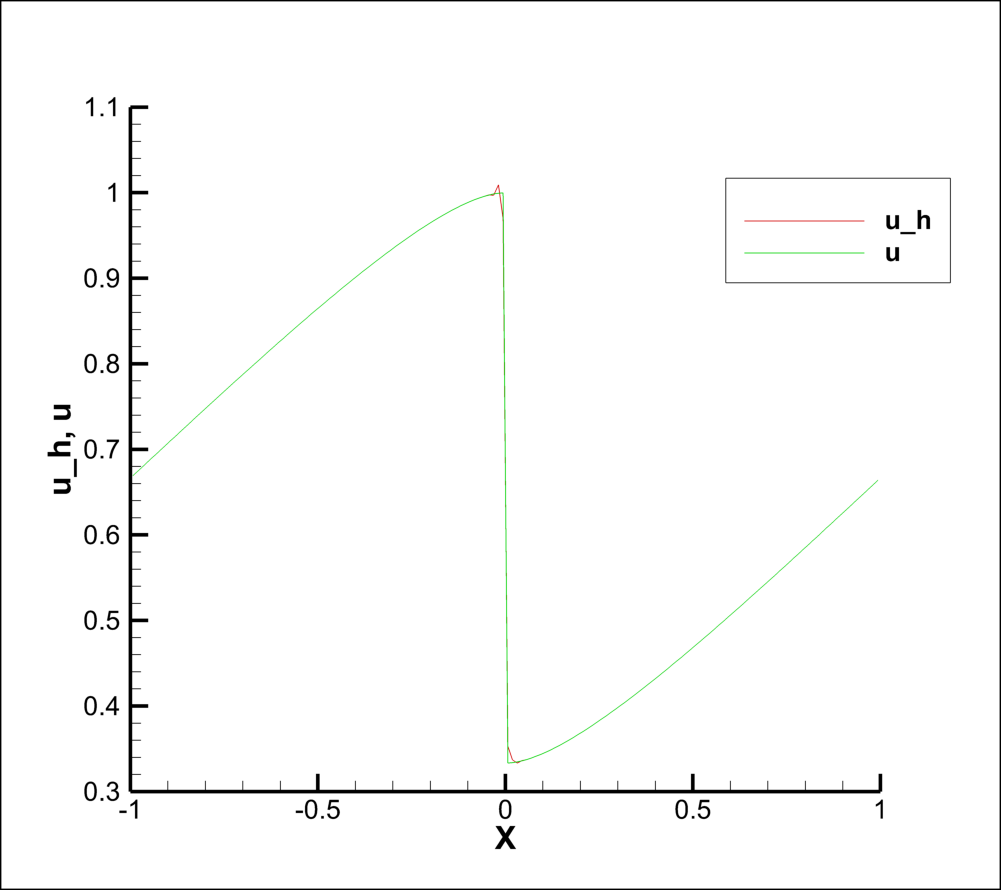
\includegraphics[width=5cm]{pics/DG_P1.png}
		}
		\quad
		\subfigure[$P^1$ without limiter zoom in]{
			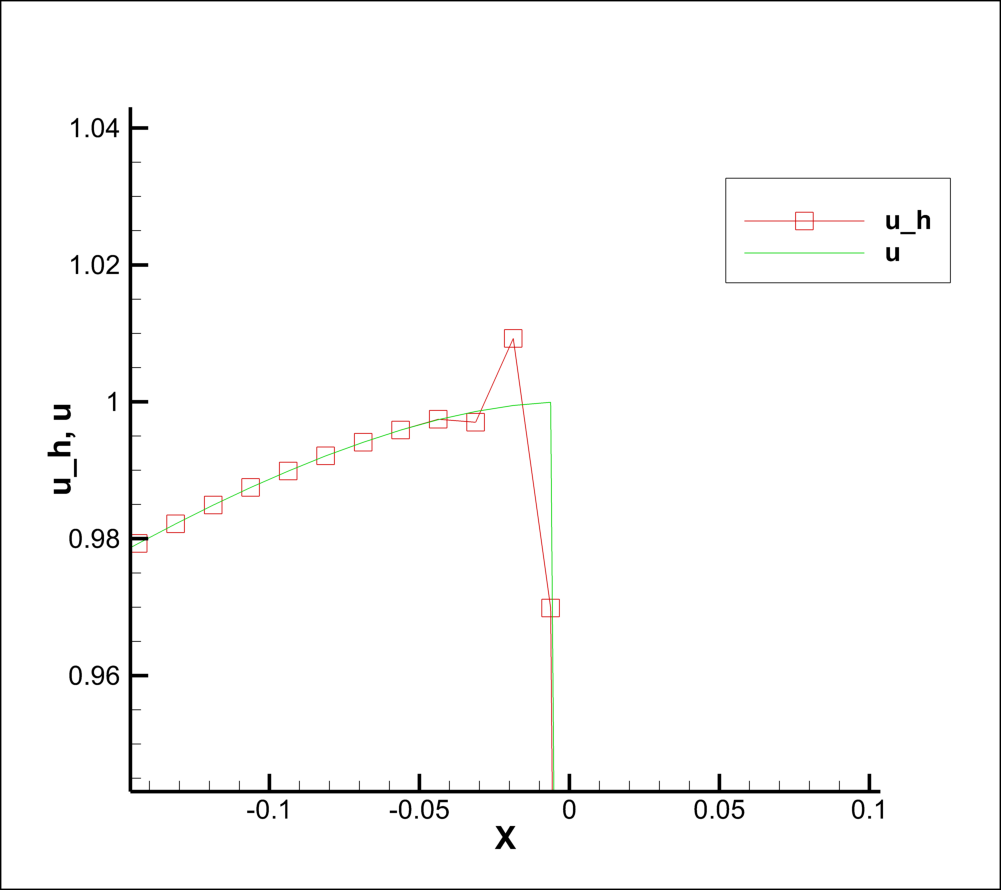
\includegraphics[width=5cm]{pics/DG_P1zoomin.png}
		}
	\quad
	\subfigure[$P^2$ without limiter]{
		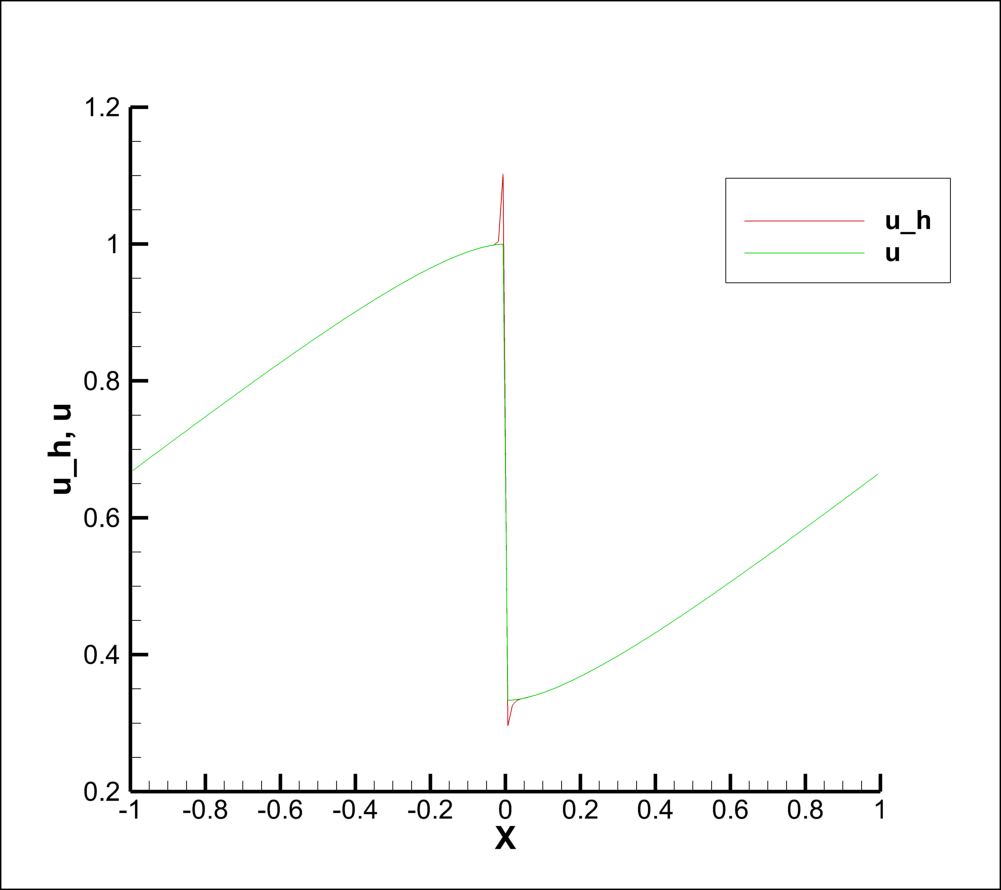
\includegraphics[width=5cm]{pics/DG_P2.png}
	}
	\quad
	\subfigure[$P^2$ without limiter zoom in]{
		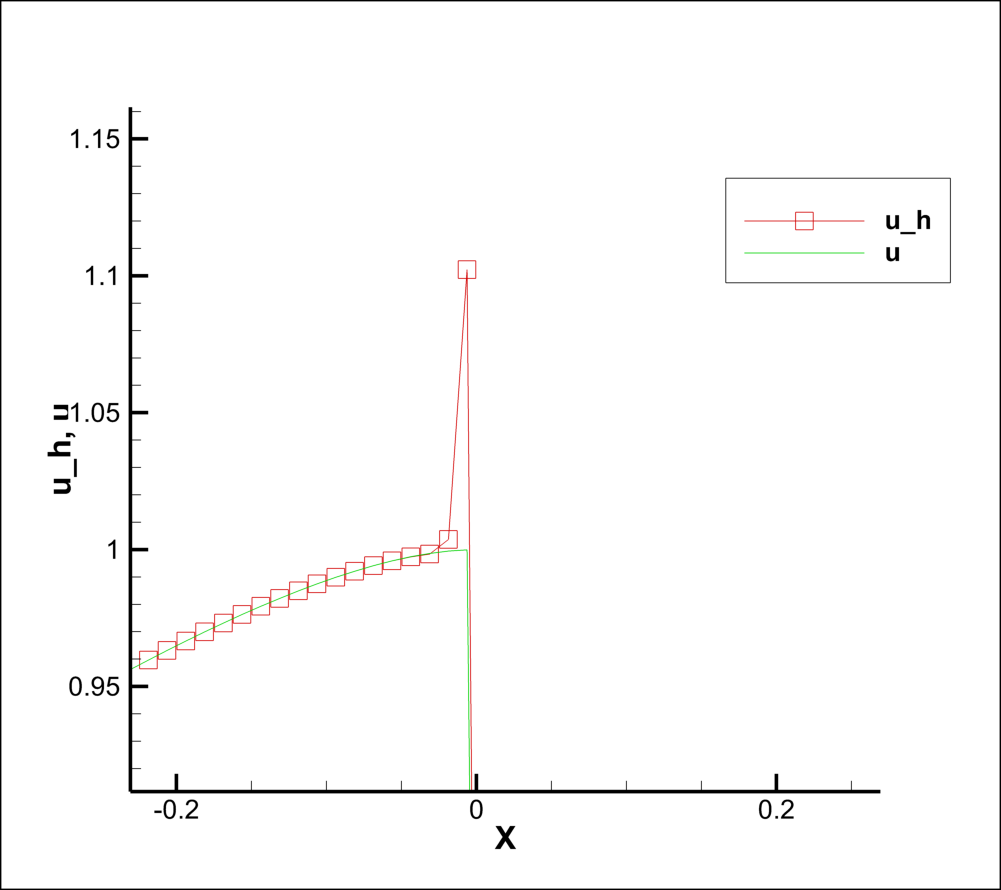
\includegraphics[width=5cm]{pics/DG_P2zoomin.png}
	}
	\caption{DG without limiter at $T=1.5$}
	\end{figure}

	当使用TVD、TVB、MPP限制器时,得到的结果见图\ref{TVD}、\ref{TVB}、\ref{MPP}:
	\begin{figure}[htbp]
		\centering
		\subfigure[$P^1$ with TVD limiter]{
			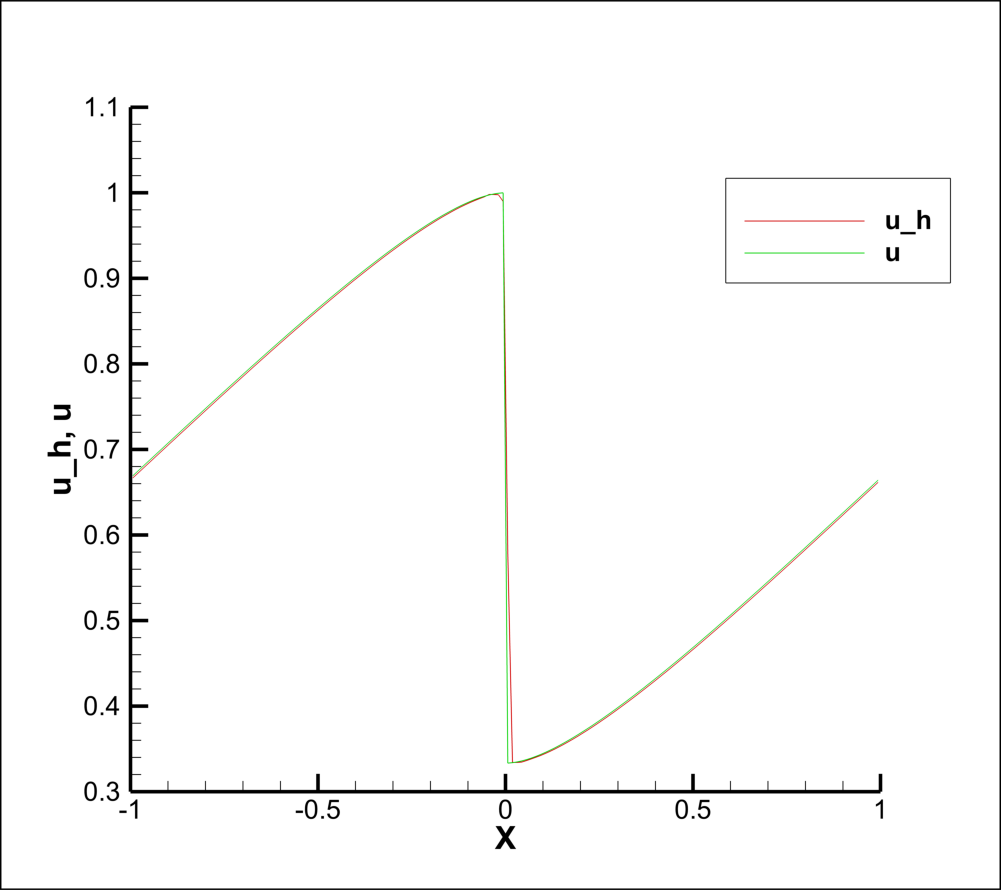
\includegraphics[width=5cm]{pics/TVD_P1.png}
		}
		\quad
		\subfigure[$P^1$ with TVD limiter zoom in]{
			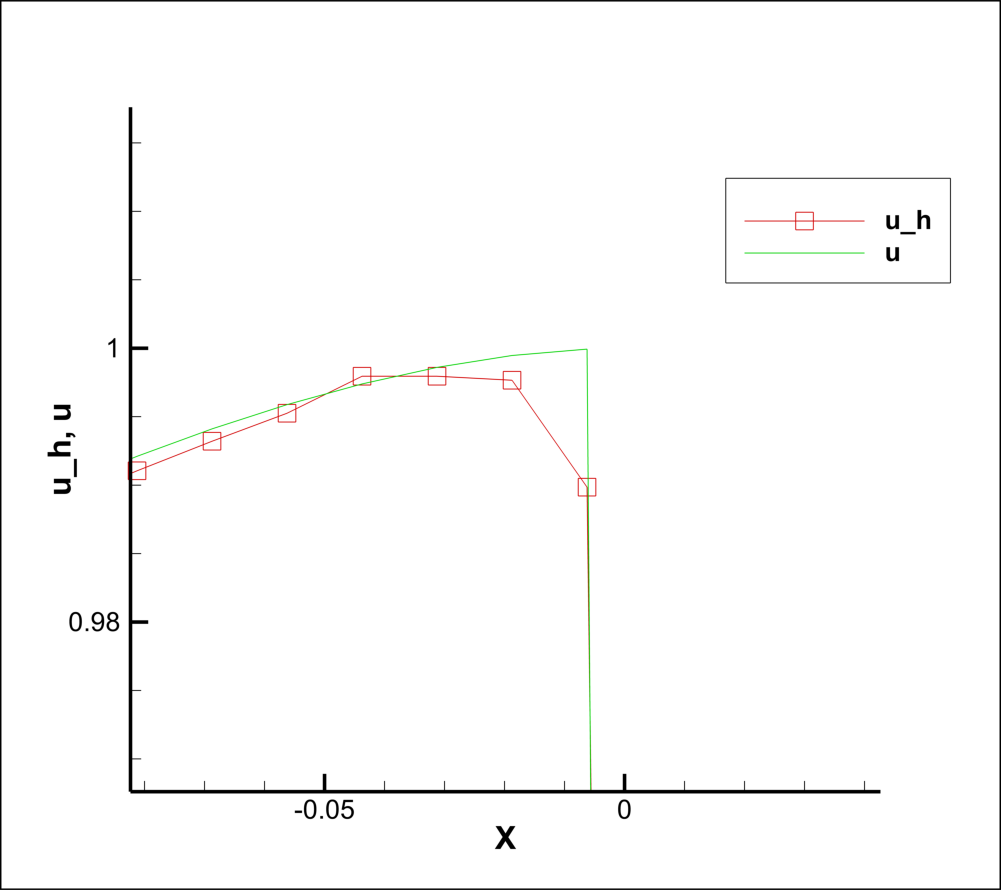
\includegraphics[width=5cm]{pics/TVD_P1zoomin.png}
		}
		\quad
		\subfigure[$P^2$ with TVD limiter]{
			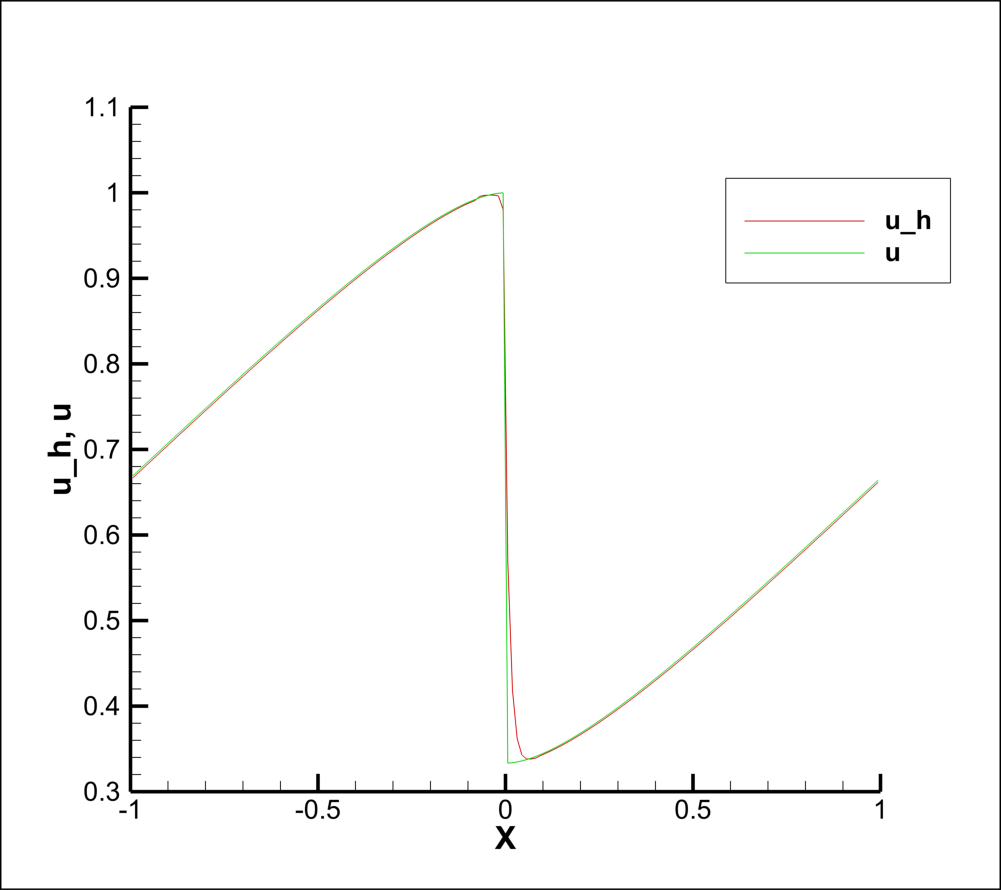
\includegraphics[width=5cm]{pics/TVD_P2.png}
		}
		\quad
		\subfigure[$P^2$ with TVD limiter zoom in]{
			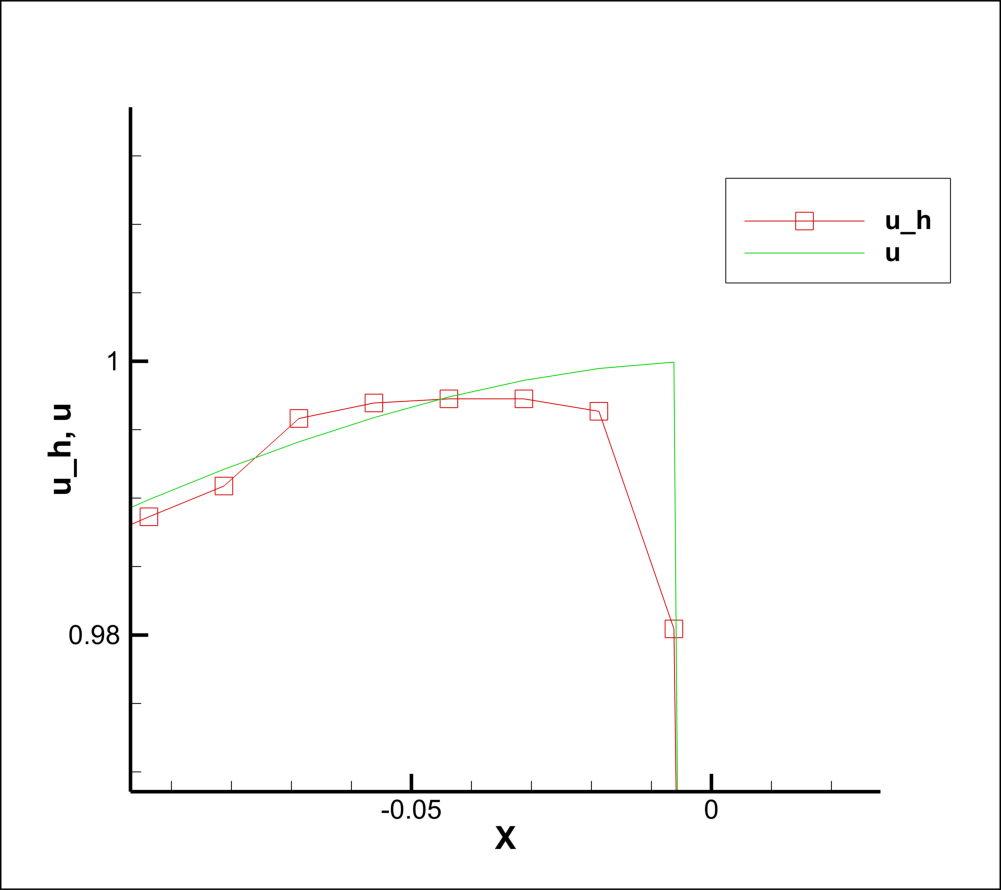
\includegraphics[width=5cm]{pics/TVD_P2zoomin.png}
		}
		\caption{DG with TVD liniter at $T=1.5$}
		\label{TVD}
	\end{figure}


	\begin{figure}[htbp]
		\centering
		\subfigure[$P^1$ with TVB limiter]{
			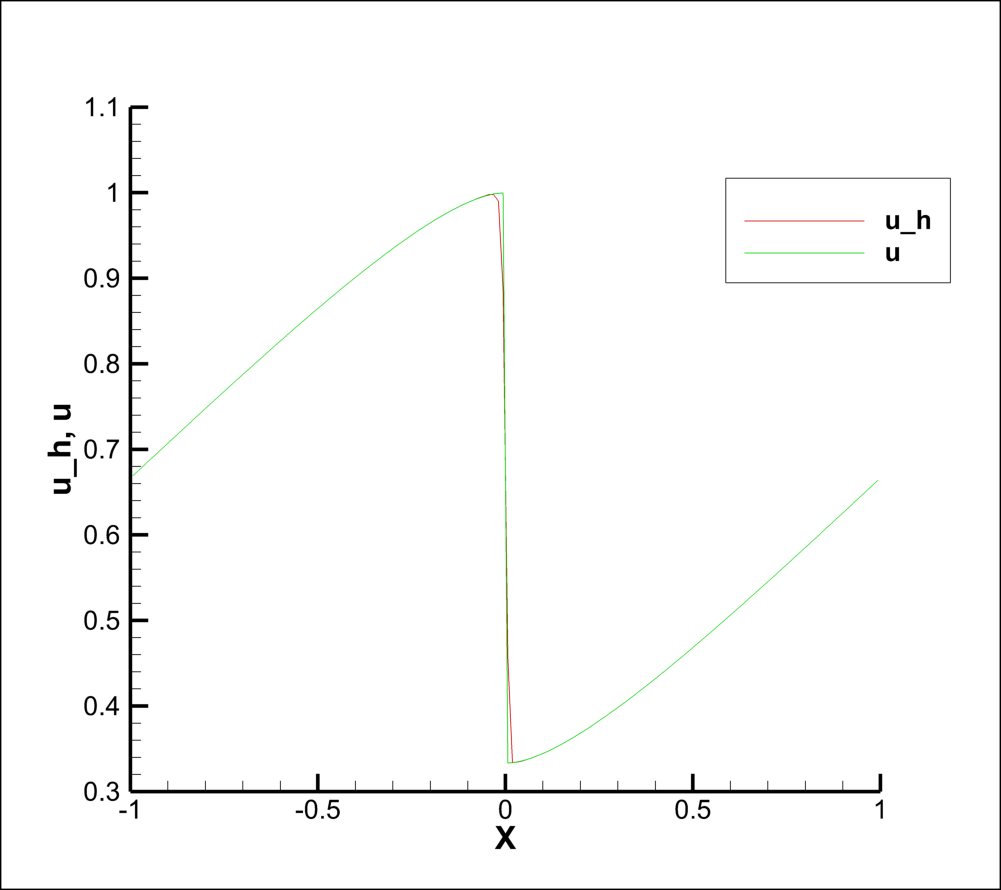
\includegraphics[width=5cm]{pics/TVB_P1.png}
		}
		\quad
		\subfigure[$P^1$ with TVB limiter zoom in]{
			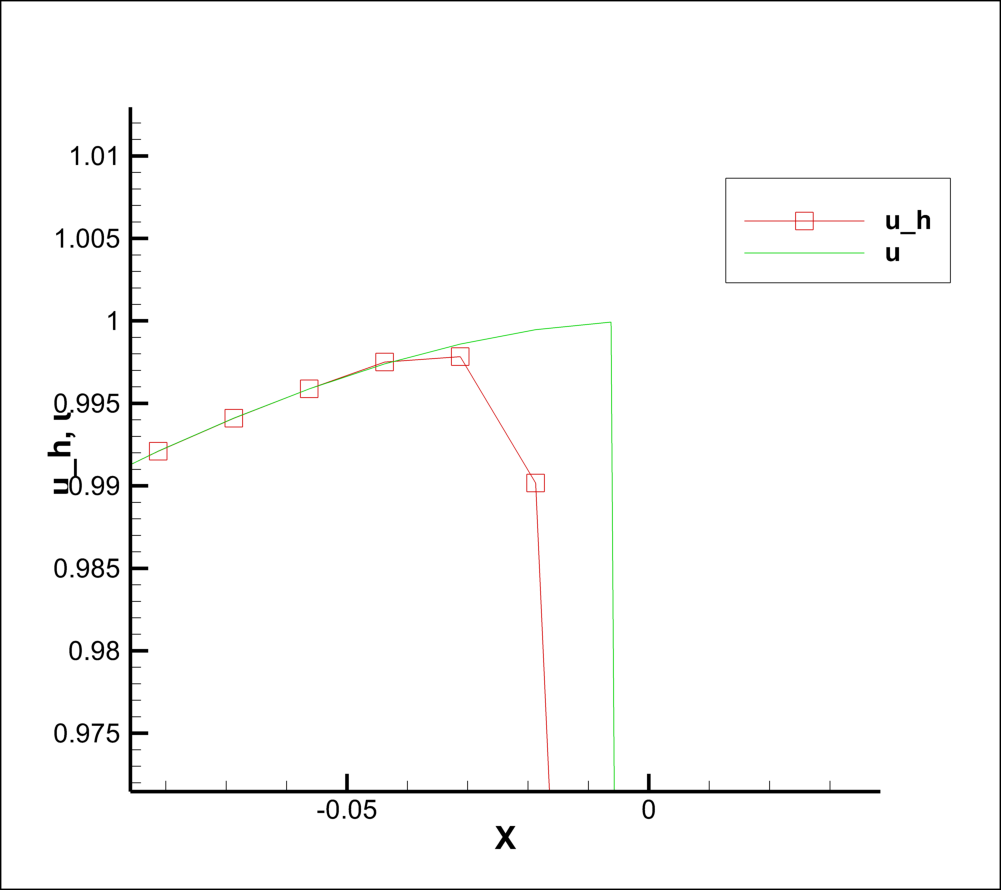
\includegraphics[width=5cm]{pics/TVB_P1zoomin.png}
		}
		\quad
		\subfigure[$P^2$ with TVB limiter]{
			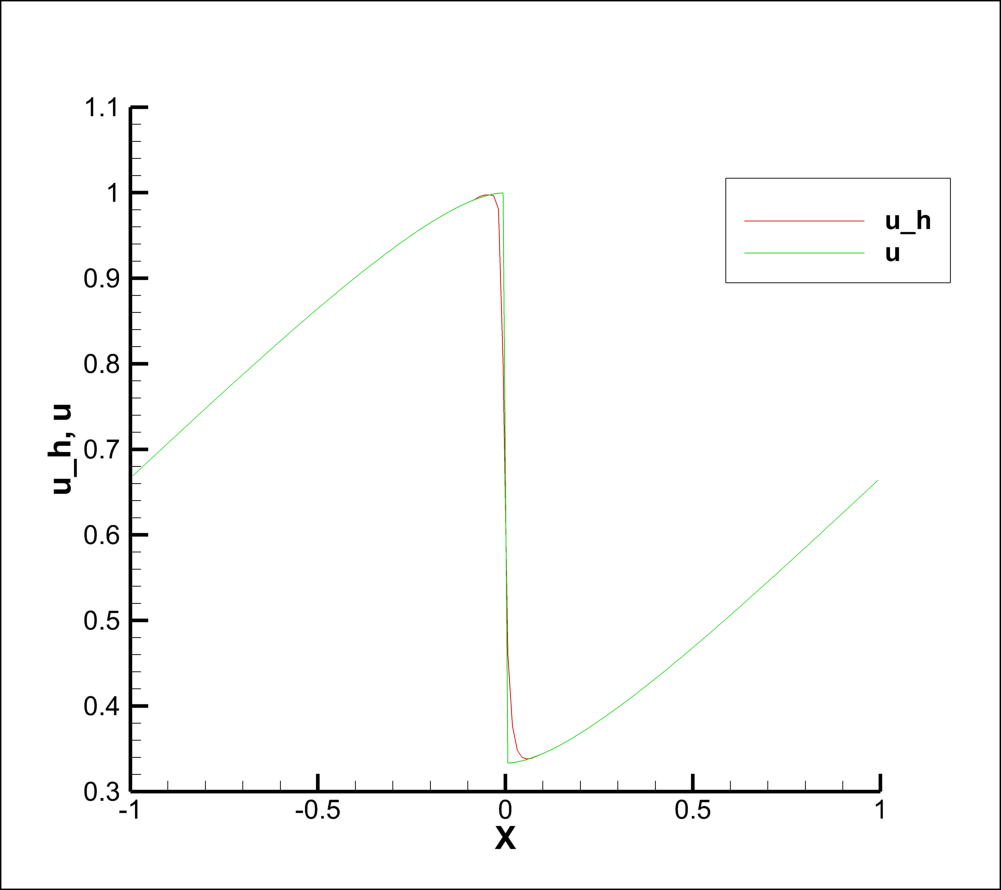
\includegraphics[width=5cm]{pics/TVB_P2.png}
		}
		\quad
		\subfigure[$P^2$ with TVB limiter zoom in]{
			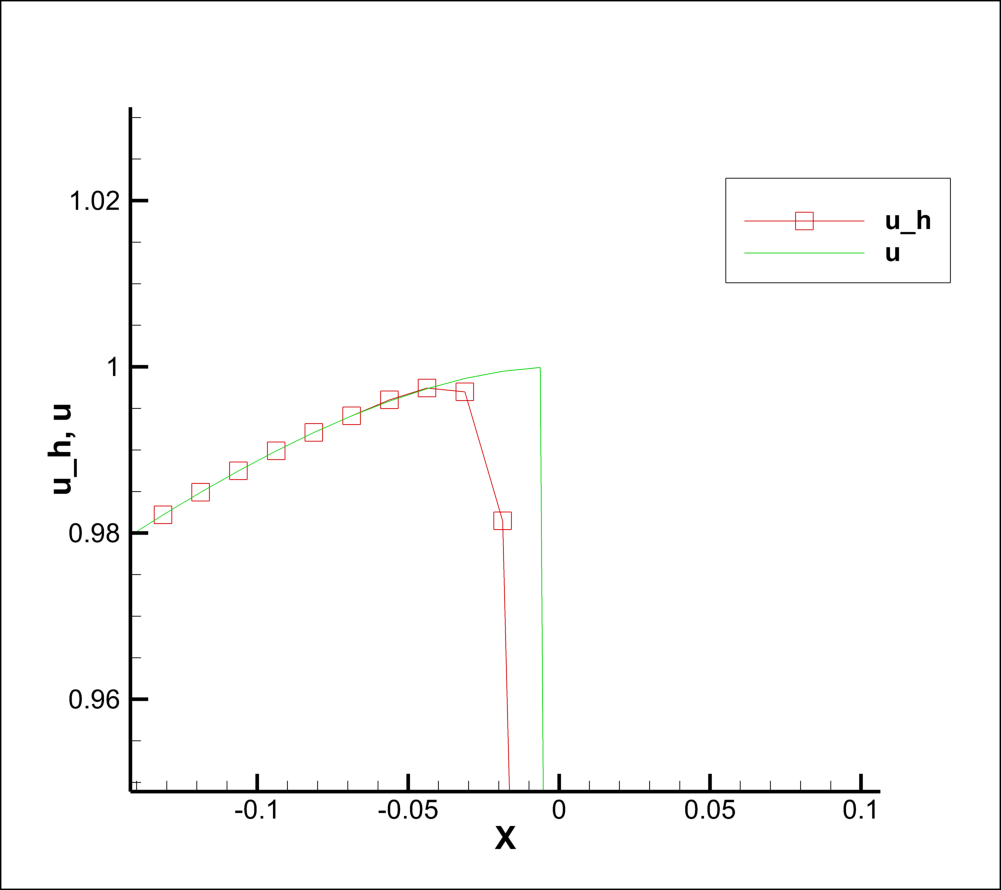
\includegraphics[width=5cm]{pics/TVB_P2zoomin.png}
		}
		\caption{DG with TVB liniter at $T=1.5$}
		\label{TVB}
	\end{figure}

	\begin{figure}[htbp]
		\centering
		\subfigure[$P^1$ with MPP limiter]{
			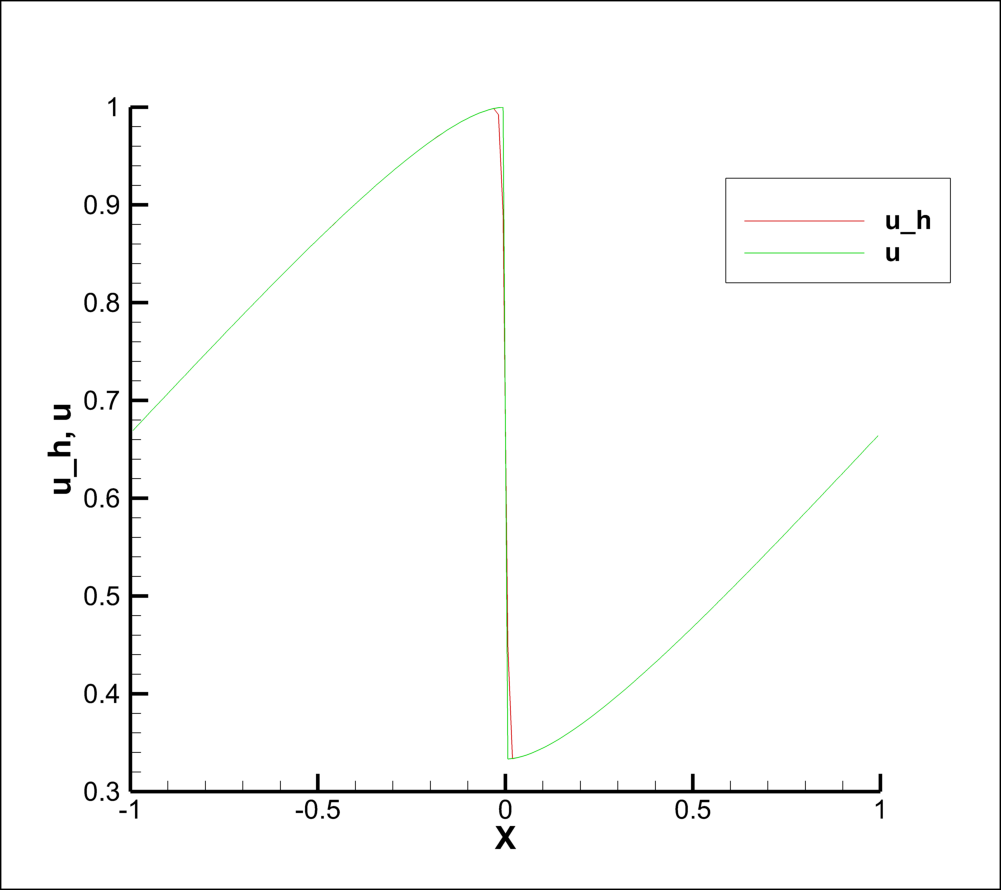
\includegraphics[width=5cm]{pics/MPP_P1.png}
		}
		\quad
		\subfigure[$P^1$ with MPP limiter zoom in]{
			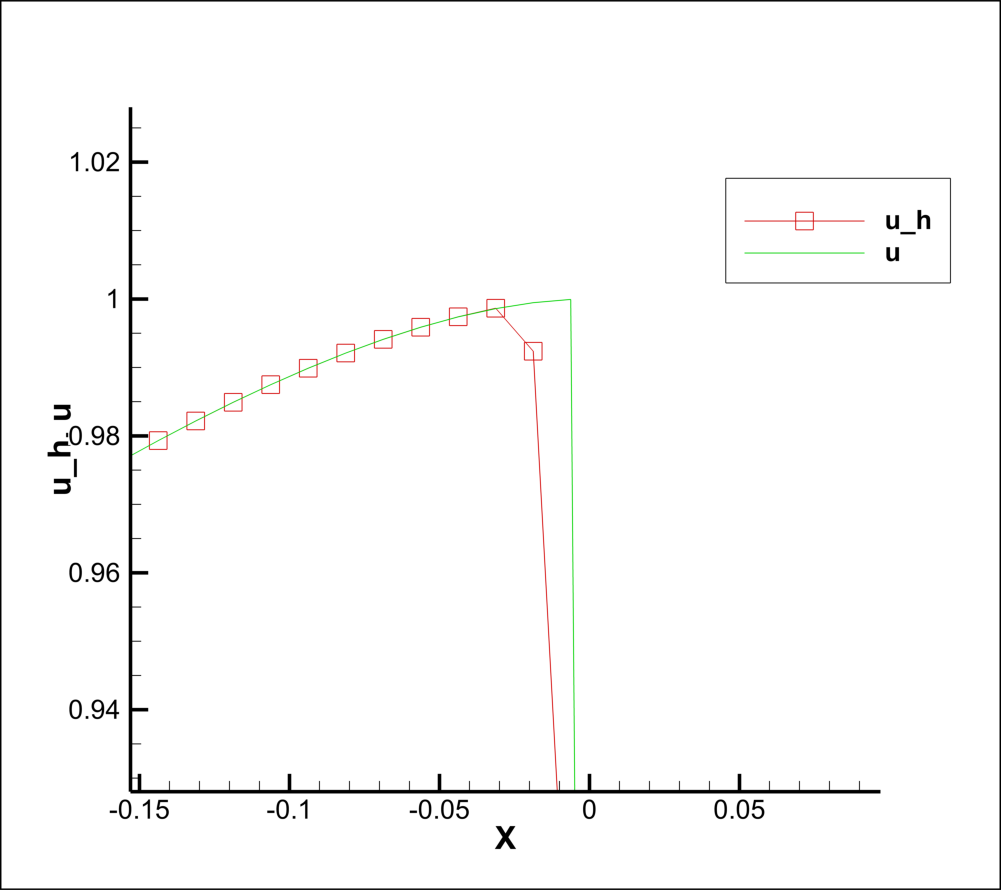
\includegraphics[width=5cm]{pics/MPP_P1zoomin.png}
		}
		\quad
		\subfigure[$P^2$ with MPP limiter]{
			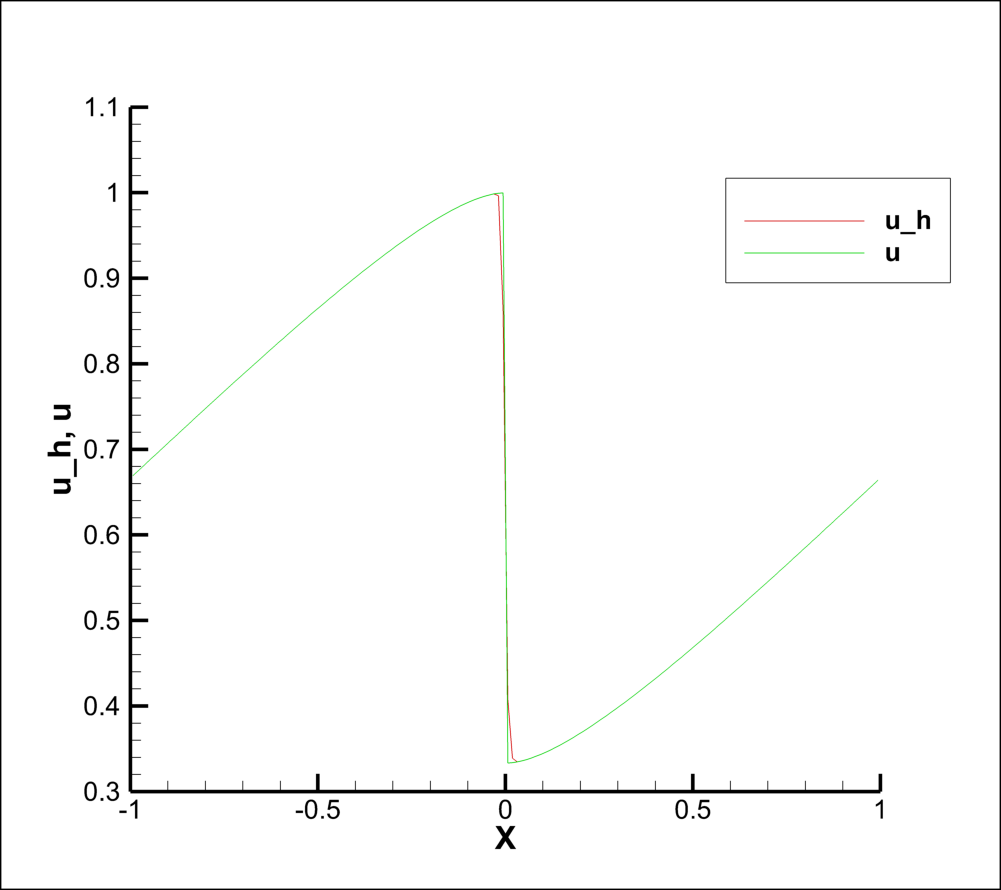
\includegraphics[width=5cm]{pics/MPP_P2.png}
		}
		\quad
		\subfigure[$P^2$ with MPP limiter zoom in]{
			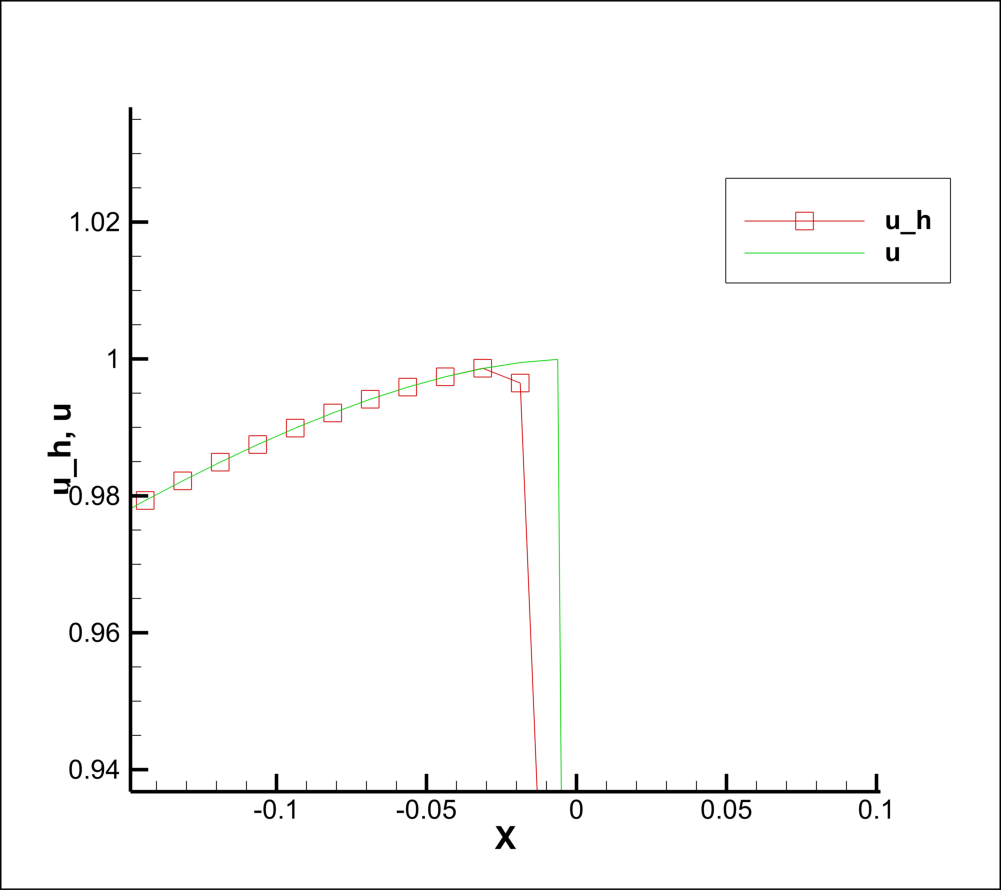
\includegraphics[width=5cm]{pics/MPP_P2zoomin.png}
		}
		\caption{DG with MPP liniter at $T=1.5$}
		\label{MPP}
	\end{figure}

	\section{分析}
	
	当$T=0.4$时,真解没有间断,限制器都保持了较高的收敛阶。当$k=1$时,TVD、TVB、MPP限制器在$L^2$范数下都保持了没有限制器时DG格式的二阶收敛阶,在$L^\infty$范数下,只有添加了TVD限制器的结果对收敛阶有较大的影响,其他限制器的收敛阶都在二阶左右。当$k=2$时,TVD限制器在$L^2$和$L^\infty$范数下的表现都不是很好,原本三阶的精度在添加TVD限制器后最高不会超过二阶。但是TVB和MPP限制器仍然能够保持接近三阶的高精度。这种情况主要是由于在真解的极值点附近TVD限制器最高只能有一阶精度造成的,而TVB和MPP限制器放宽了对数值解的要求。
	
	当$T=1.5$时会出现激波,在$x=0$的位置会出现间断,DG格式求得的数值解在间断处会产生振荡现象。TVD、TVB、MPP限制器都能消除振荡,但是效果不同。TVD限制器在间断附近耗散比较大, 和真解不是非常吻合。TVB和MPP限制器对真解的逼近效果比较好。
	
	\section{代码}
	本次报告程序使用C++编译。
	
	\appendix
	
	\begin{lstlisting}
	#include <iostream>
	#include <cmath>
	#include <fstream>
	using namespace std;
	
	//先定义一些全局的变量
	const int n = 160;   //划分单元个数
	const int k = 1;    //多项式最高次项次数
	const double h = (double) 2/n;    //空间步长
	const double dt = (double) h * h  ;    //时间步长
	const double pi = 3.1415926;
	
	double p[n+1];  //节点位置,p_j = j * h = x_{j+1/2}, j =0,1, ..., n
	//存储不变的系数矩阵
	
	const double lobattopoint[5] = {-1.0, -0.6546536707079771, 0, 0.6546536707079771, 1.0};
	const double lobattoco[5] = {0.1, 0.5444444444444444, 0.7111111111111111, 0.5444444444444444, 0.1};
	
	//*************函数声明*************//
	double u_0(double y);   //初值
	double u_exact(double y, double t);   //真解
	double f(double y); //通量函数
	double phi(int l, double y);    //参考单元基函数
	double** initial();   //计算初始时刻u_j
	double* cellaverage(double** un); //求单元平均
	double minimal(double a1, double a2, double a3);
	double** modify(double** un);
	double flux(double ul, double ur);  //数值通量计算
	double** L(double** ut);   //用于计算RK的函数,u_t= F(u)
	double** RK22(double** un);    //2步二阶RK
	double** RK33(double** un);
	double** RK(int k, double** un);
	//************声明完毕**************//
	
	int main()
	{
	int i, j, l;
	double t, temp1, temp2, norm1, norm2, xi;
	double T = 1.5;
	double** u1 = new double* [n];
	double** u2 = new double* [n];
	for (i=0; i<n; i++)
	{
	u1[i] = new double [k+1];
	u2[i] = new double [k+1];
	}
	for (j=0; j<=n; j++)
	{
	p[j] = j * h - 1;
	}
	
	
	u1 = initial();
	t = 0;
	while(t<T - 1e-10)
	{
	
	t = t + dt;
	u2 = RK(k,u1);
	
	u1 = u2;
	cout<<t<<endl;
	}
	
	//*
	norm1 = 0;
	norm2 = 0;
	for (j=1; j<=n; j++)
	{
	
	for (i=0; i<5; i++)
	{
	xi = lobattopoint[i];
	temp1 = 0;
	for (l=0; l<=k; l++)
	{
	temp1 = temp1 + u1[j-1][l] * phi(l,xi);
	}
	
	temp2 = h * (xi + 1) / 2. + p[j-1];
	temp1 = u_exact(temp2,T) - temp1;
	
	if (abs(temp1) > norm2)
	{
	norm2 = abs(temp1);
	}
	
	temp1 = temp1 * temp1;
	norm1 = norm1 + lobattoco[i] * temp1;
	}
	
	}
	norm1 = norm1 * h / 2.;
	norm1 = sqrt(norm1);
	cout<<"L2="<<norm1<<endl<<"Linf="<<norm2<<endl;//*/
	
	{
	const char* fn = "DGLecture\\homework4\\TVD.plt";
	remove(fn);
	fstream f, f1;
	f.open(fn, ios::out | ios :: app);
	f<<"VARIABLES="<<"X"<<","<<"u_h"<<","<<"u"<<endl;
	for (j=1; j<=n; j++)
	{
	temp1 = 0;
	temp2 = 0;
	for (l=0; l<=k; l++)
	{
	temp1 = temp1 + u1[j-1][l] * phi(l,-1);
	temp2 = temp2 + u1[j-1][l] * phi(l,1);
	}
	f<<"\t"<<(p[j-1] + p[j])/2.0<<"\t"<<temp1<<"\t"<<u_exact((p[j-1] + p[j])/2.0,T)<<endl;
	
	}
	f.close();
	}
	
	for (i=0; i<n; i++)
	{
	delete[] u1[i];
	delete[] u2[i];
	}
	delete[] u1;
	delete[] u2;
	
	system("pause");
	}
	
	double u_0(double y)
	{
	return sin(pi*y) / 3.0 + 2.0 / 3.0 ;
	}
	
	double u_exact(double y, double t)
	{
	int time=1;
	double ans, xi1=0, xi2=0.1;
	double e = 1e-6;
	
	//if (t==1.5)  //1.5时刻发生激波,单独算
	{
	if (y < -1+2*t/3.0)
	{
	y = y+2;
	}
	}
	
	while(abs(xi1 - xi2)>e)
	{
	xi1 = xi2;
	xi2 = xi1 + ( y - u_0(xi1) * t - xi1 ) / (t * pi * cos(pi*xi1)/3.0 + 1);
	time++;
	if (time > 10000)
	{
	cout<<"error"<<endl;
	cout<<y<<endl;
	break;
	}
	}
	ans = u_0(xi2);
	
	return ans;
	}
	
	double f(double y)
	{
	return y * y /2;
	}
	
	double phi(int l, double y)
	{
	if (l==0)
	{
	return 1;
	}
	else if (l == 1)
	{
	return y;
	}
	else if (l == 2)
	{
	return (3*y*y - 1)/2;
	}
	else{
	return 0;
	}
	}
	
	double** initial()
	{
	double ans, temp;
	int j, l, m;
	double** ut = new double* [n];
	double* Bt = new double [n];
	for (j=0; j<n; j++)
	{
	ut[j] = new double [k+1];
	}
	
	for (j=1; j<=n; j++)
	{
	for (m=0; m<=k; m++)
	{
	ans = 0;
	for (l=0; l<5; l++)
	{
	temp = h * (lobattopoint[l] + 1)/2 + p[j-1];
	ans = ans + lobattoco[l] * u_0(temp) * phi(m,lobattopoint[l]);
	}
	ans = ans / 2;
	Bt[m] = ans;
	}
	
	double A[3][3] = {{1,0,0},{0,3,0},{0,0,5}};
	for (m=0; m<=k ;m++)
	{
	ut[j-1][m] = 0;
	for (l=0; l<=k; l++)
	{
	ut[j-1][m] = ut[j-1][m] + A[m][l] * Bt[l];
	}
	}
	
	}
	
	delete[] Bt;
	
	return ut;
	}
	
	double* cellaverage(double** un)
	{
	int j, l;
	double* ca = new double[n];
	double D[3] ;
	
	for (j=0; j<3; j++)
	{
	D[j] =0;
	for (l=0; l<5; l++)
	{
	D[j] = D[j] + lobattoco[l]*phi(j,lobattopoint[l]);
	}
	}
	for (j=1; j<=n; j++)
	{
	ca[j-1] = 0;
	for (l=0; l<=k; l++)
	{
	ca[j-1] = ca[j-1] + D[l] * un[j-1][l];
	}
	ca[j-1] = ca[j-1] / 2.0;
	}
	
	return ca;
	}
	
	double minimal(double a1, double a2, double a3)
	{
	double ans, temp;
	if (a1 > 0)
	{
	if (a2 > 0 && a3 > 0)
	{
	temp = min(a2,a3);
	ans = min(temp, a1);
	}
	else{
	ans = 0;
	}
	}
	else{
	if (a2 <0 && a3 <0)
	{
	temp = min(abs(a2),abs(a3));
	ans = - min(abs(a1), temp);
	}
	else{
	ans = 0;
	}
	}
	
	return ans;
	}
	
	double** modify(double** un)
	{
	int j, l, r;
	double** mod = new double* [n];
	for (j=1; j<=n; j++)
	{
	mod[j-1] = new double [k+1];
	}
	
	double u1, u2;
	double* ca = new double [n];
	
	ca = cellaverage(un);
	
	for (j=1; j<=n; j++)
	{
	u1 = 0;
	u2 = 0;
	for (l=0; l<=k; l++)
	{
	u1 = u1 + un[j-1][l] * phi(l,1);
	u2 = u2 + un[j-1][l] * phi(l,-1);
	}
	
	u1 = u1 - ca[j-1];
	u2 = ca[j-1] - u2;
	
	if (j == 1)
	{
	r = j;
	l = n-1;
	}
	else if(j == n)
	{
	r = 0;
	l = j-2;
	}
	else{
	r = j;
	l = j-2;
	}
	u1 = minimal(u1, ca[r] - ca[j-1], ca[j-1]- ca[l]);
	u2 = minimal(u2, ca[r] - ca[j-1], ca[j-1]- ca[l]);
	
	u1 = u1 + ca[j-1];
	u2 = ca[j-1] - u2;
	
	if ( k == 1)
	{
	mod[j-1][0] = (u1 + u2)/2.0;
	mod[j-1][1] = (u1 - u2)/2.0;
	}
	else if (k == 2)
	{
	mod[j-1][0] = ca[j-1];
	mod[j-1][1] = (u1 - u2)/2.0;
	mod[j-1][2] = (u1 + u2)/2.0 - ca[j-1];
	}
	}
	
	delete[] ca;
	return mod;
	}
	
	double flux(double ul, double ur)
	{
	double ans, alpha;
	int i, l;
	if ( ul <= ur)
	{
	//ans = f(ul);  //Godnov
	alpha = ur; //Lax-Friedrichs
	}
	else{
	//ans = f(ul);
	alpha = ul;
	}
	
	ans = f(ul) + f(ur) - alpha * (ur - ul);
	ans = ans * 0.5;
	
	return ans;
	}
	
	double** L(double** ut)
	{
	int i, j, l, m, p, q;
	double ul, ur;
	double** ans = new double* [n];
	for (i=0; i<n; i++)
	{
	ans[i] = new double [k+1];
	}
	
	double A[3] = {1,3,5};
	double B[3][3][3] = {{{0,0,0},{0,0,0},{0,0,0}}, {{2,0,0},{0,2.0/3.0,0},{0,0,2.0/5.0}}, {{0,2,0},{2,0,4.0/5.0},{0,4.0/5.0,0}}};
	
	
	for (j=1; j<=n; j++)
	{
	for (m=0; m<=k; m++)
	{
	ans[j-1][m] = 0;
	
	for (p=0; p<=k; p++)
	{
	for (q=0; q<=k; q++)
	{
	ans[j-1][m] = ans[j-1][m] + ut[j-1][p] * B[m][p][q] * ut[j-1][q];
	}
	}
	ans[j-1][m] = ans[j-1][m] / 2;
	
	//计算第一个数值通量
	{
	ul = 0;
	ur = 0;
	q = j;
	if (q == n)
	{
	q = 0;
	}
	for (l=0; l<=k; l++)
	{
	ul = ul + ut[j-1][l] * phi(l,1);
	ur = ur + ut[q][l] * phi(l,-1);
	}
	ans[j-1][m] = ans[j-1][m] - flux(ul,ur) * phi(m,1);
	
	}
	
	//计算第二个数值通量
	{
	ul = 0;
	ur = 0;
	
	p = j-2;
	if ( p == -1)
	{
	p = n-1;
	}
	for (l=0; l<=k; l++)
	{
	ul = ul + ut[p][l] * phi(l,1);
	ur = ur + ut[j-1][l] * phi(l,-1);
	}
	ans[j-1][m] = ans[j-1][m] + flux(ul,ur) * phi(m,-1);
	}
	
	ans[j-1][m] = ans[j-1][m] * A[m] / h;
	}
	}
	
	return ans;
	}
	
	double** RK22(double** un)
	{
	int j,l,m;
	double ul;
	double** ans = new double* [n];
	for (j=0; j<n; j++)
	{
	ans[j] = new double [k+1];
	}
	double** u0 = new double* [n];
	double** u1 = new double* [n];
	double** u2 = new double* [n];
	
	for (j=0; j<n; j++)
	{
	u0[j] = new double [k+1];
	u1[j] = new double [k+1];
	u2[j] = new double [k+1];
	}
	
	for (j=1; j<=n; j++)
	{
	for (l=0; l<=k; l++)
	{
	u0[j-1][l] = un[j-1][l];
	}
	}
	u0 = modify(u0);
	
	u1 = L(u0);
	for (j=1; j<=n; j++)
	{
	for (l=0; l<=k; l++)
	{
	u1[j-1][l] = u1[j-1][l] * dt  + u0[j-1][l];
	}
	}
	u1 = modify(u1);
	
	
	u2 = L(u1);
	for (j=1; j<=n;j++)
	{
	for (l=0; l<=k; l++)
	{
	u2[j-1][l] = u0[j-1][l] * 0.5 + u1[j-1][l] * 0.5 + u2[j-1][l] * 0.5 * dt;
	ans[j-1][l] = u2[j-1][l];
	}
	}
	ans = modify(ans);
	
	
	delete[] u0;
	delete[] u1;
	delete[] u2;
	
	return ans;
	}
	
	double** RK33(double** un)
	{
	int j,l,m;
	double ul;
	double** ans = new double* [n];
	for (j=0; j<n; j++)
	{
	ans[j] = new double [k+1];
	}
	double** u0 = new double* [n];
	double** u1 = new double* [n];
	double** u2 = new double* [n];
	double** u3 = new double* [n];
	
	for (j=0; j<n; j++)
	{
	u0[j] = new double [k+1];
	u1[j] = new double [k+1];
	u2[j] = new double [k+1];
	u3[j] = new double [k+1];
	}
	
	for (j=1; j<=n; j++)
	{
	for (l=0; l<=k; l++)
	{
	u0[j-1][l] = un[j-1][l];
	}
	}
	u0 = modify(u0);
	
	u1 = L(u0);
	for (j=1; j<=n; j++)
	{
	for (l=0; l<=k; l++)
	{
	u1[j-1][l] = u1[j-1][l] * dt  + u0[j-1][l];
	}
	}
	u1 = modify(u1);
	
	
	u2 = L(u1);
	for (j=1; j<=n;j++)
	{
	for (l=0; l<=k; l++)
	{
	u2[j-1][l] = u0[j-1][l] * 3 / 4 + u1[j-1][l] /4 + u2[j-1][l] * dt / 4;
	}
	}
	u2 = modify(u2);
	
	u3 = L(u2);
	for (j=1; j<=n; j++)
	{
	for (l=0; l<=k; l++)
	{
	u3[j-1][l] = u0[j-1][l] / 3 + 2 * u2[j-1][l] / 3 + 2 * dt * u3[j-1][l] /3;
	ans[j-1][l] = u3[j-1][l];
	}
	}
	ans = modify(ans);
	
	
	delete[] u0;
	delete[] u1;
	delete[] u2;
	delete[] u3;
	
	return ans;
	}
	
	double** RK(int k, double** un)
	{
	double** u2;
	if ( k == 1 )
	{
	u2 = RK22(un);
	}
	else if (k == 2)
	{
	u2 = RK33(un);
	}
	else{
	;
	}
	
	return u2;
	}
	\end{lstlisting}
	\end{document}